\chapter{Introduction}


% ***
% Plan
%
% mention mcrt, what it is
% examples of its use in tissue optics
% pdf, islas work, port wine stains, radiation therapy
% real power is that can be used as a form of personalised medicine
%
%
% ***
This thesis is concerned with the development of several \gls*{mcrt} algorithms for biophotonic and medical applications.
The \gls*{mcrt} method allows the simulation of light propagation through turbid media whilst undergoing multiple anisotropic scattering, absorption and a range of other micro-physics (see~\cref{sec:mcrt} for full discussion of the theory).
\Gls*{mcrt} was invented at the end of World War II for the purpose of calculating the paths of neutrons through various media~\cite{montybeg1,eckhardt1987stan,anderson1986metropolis,ulam1947statistical}.
As the codes developed around this period focused on modelling the transport of protons, gamma rays and other nuclear particles, it was a small leap to modelling the dose received by a patient undergoing radiation therapy~\cite{ellett1964gamma}.
However, the jump to modelling light transport in skin would take a further two decades~\cite{wilson1983monte}, and another decade until it became popular and the \textit{de-facto} gold standard in light tissue interaction modelling~\cite{wang1995mcml,key1991monte}.
It has since been used to optimise photo-dynamic therapy, quantifying DNA damage from UV light sources, and modelling treatment of port wine stain removal amongst various other medical treatments and diagnosis methods~\cite{barnard2018quantifying,smithies1995modelling,campbell2015monte}.
The real power of the \gls*{mcrt} method is that it allows the model to be tailored to the patient.
This means the medical treatment can be personalised to each individual patient rather than an average corpus of patients.\\


Personalised medicine entails having fine grained knowledge of the patient down to the genome level, to understand how various drugs or treatments will affect the patient.
One particular area of research in personalised medicine is into the so called ``digital twin''.
A digital twin as defined by A. El Saddik as~\cite{el2018digital}:

\medskip
``... is a digital replica of a living or non-living physical entity.''
\medskip

\noindent Digital twins are currently heavily used in engineering to predict when various machinery will need to undergo maintenance.
Digital twins operate by modelling their physical counterpart.
This model is updated via information from their physical counterpart which allows the digital twin to predict it's physical counterparts future behaviour.
Companies like Phillips use this in their MRI machines to help schedule downtime, and predict which parts the engineer will need on site, both of which minimises the downtime of the machine which is important for the hospital or clinic~\cite{henkvanhouten2018}.

At the heart of the digital twin method is the ability to accurately model the object or living thing being studied.
This can be straightforward when the twin in question is a machine, as sensors can usually be attached to the various components to get feedback on the machine's operation.
Machines also have the bonus of (normally) being well understood so that modelling them is usually relatively straightforward.
However, this is not as easy when dealing with living systems.
First, we still do not have a complete understanding of the biology within humans.
Therefore, modelling a human accurately is not possible as various assumptions and approximations have to be made.
Second, to get accurate information on what is happening inside a patient, generally either ionising radiation needs to be used or cameras inserted into the patient.
Both of these cannot be done for indefinite periods without causing harm or discomfort.
Therefore, continuous information on the inner functions of the body is not possible.
One area where information is more readily available is the skin.
Information on the skin function or dysfunction is normally diagnosed with light.
Light is also used in various treatments such as photodynamic therapy and tissue ablation, over various internal and external sites on the body.
Light's interaction over the whole spectrum, from the UV to the infrared, is readily modelled with techniques such as \gls*{mcrt}.
\Gls*{mcrt} allows a digital twin model of the individual patient's skin to be simulated.
This can then be used to tailor treatment regimes for the patient, or to predict treatment outcomes for specific patients.
The use of simulation techniques like \gls*{mcrt} allow testing \textit{in-silico}, and can negate the need to test on humans or animals.
\Gls*{mcrt} is already heavily used to plan radiation therapy treatments~\cite{andreo2018monte,andreo1991monte}, though this has yet to make the leap to light-tissue interaction modelling.


\section{Monte Carlo Method}\label{sec:mcmethod}
The Monte Carlo method is a numerical analysis technique based upon random numbers, which are used to calculate unknown variables in problems~\cite{cashwell1959practical,rogers1990monte}. 

The earliest use of the method is in Buffon's needle experiment of the 18$^{\text{th}}$ century~\cite{badger1994lazzarini,beckmann2015history,buffon1785histoire}. Buffon asked the question;

\medskip

``Suppose we have a floor made of parallel strips of wood, each the same width, and we drop a needle onto the floor. What is the probability that the needle will lie across a line between two strips?''

\medskip

The solution to this for a needle of length \textit{l}, a strip separation \textit{s}, $\theta$ is the angle of the needle with respect to the wood strips, and where \textit{x} is the distance from the needle to the closest line,. Then, using a simple geometrical argument, a needle crosses a strip if $x \leq \tfrac{l}{2} sin \theta$.

$x$ is distributed uniformly in [0, $\tfrac{s}{2}$], and $\theta$ in [0, $\tfrac{\pi}{2}$]. Therefore the probability density function for $x$ is $p(x)=\tfrac{2}{s}$, and $\theta$ is $p(\theta) = \tfrac{2}{\pi}$. The \gls*{pdf} is a function of a variable that gives the probability for a variable to take a given value. The \gls*{pdf} is normalised over the whole range of the variable, in this case $x$, and $\theta$.
Thus, as $x$ and $\theta$ are independent variables, giving a joint probability of $p(x,\theta) = \tfrac{4}{s \pi}$.
So the probability of a needle of length $l$ crossing a line ($l<s$) is:

\begin{equation}
P=\int_0^{\frac{\pi}{2}}\int_0^{\frac{l}{2}sin\theta}\frac{4}{s\pi}\ dx\ d\theta = \frac{2 l}{s \pi}\label{eqn:buffon}
\end{equation}


\Cref{eqn:buffon} can be used to carry out a Monte Carlo estimation of $\pi$. A simple rearrangement yields: $\pi = \tfrac{2l}{sP}$ where P is the ratio of needles crossing the line to the total number dropped. Laplace was the first to suggest that Buffon's needle experiment could be used to estimate $\pi$~\cite{beckmann2015history}. 
\Cref{fig:buffon-needle} shows an example of a simulation of Buffon's needle experiment.

\medskip

There are various different approaches to using the Monte Carlo method to obtain randomly sampled variables.
One analytical way of achieving this is the inverted sampling method.
The inverted sampling method can be summarised by the following steps for drawing a sample $X_i$ from an arbitrary PDF $p(x)$:

\medskip

1. Compute the \gls*{cdf} $P(x)=\int^{x}_{0}p(x')dx'$

2. Compute the inverse $P^{-1}(x)$

3. Obtain a uniformly distributed random number $\xi$ in the range [0.,1.)

4. Finally, compute $X_i = P^{-1}(\xi)$

\medskip

\begin{figure}[!hbp]
    \squeezeup{5.5}
    \centering
    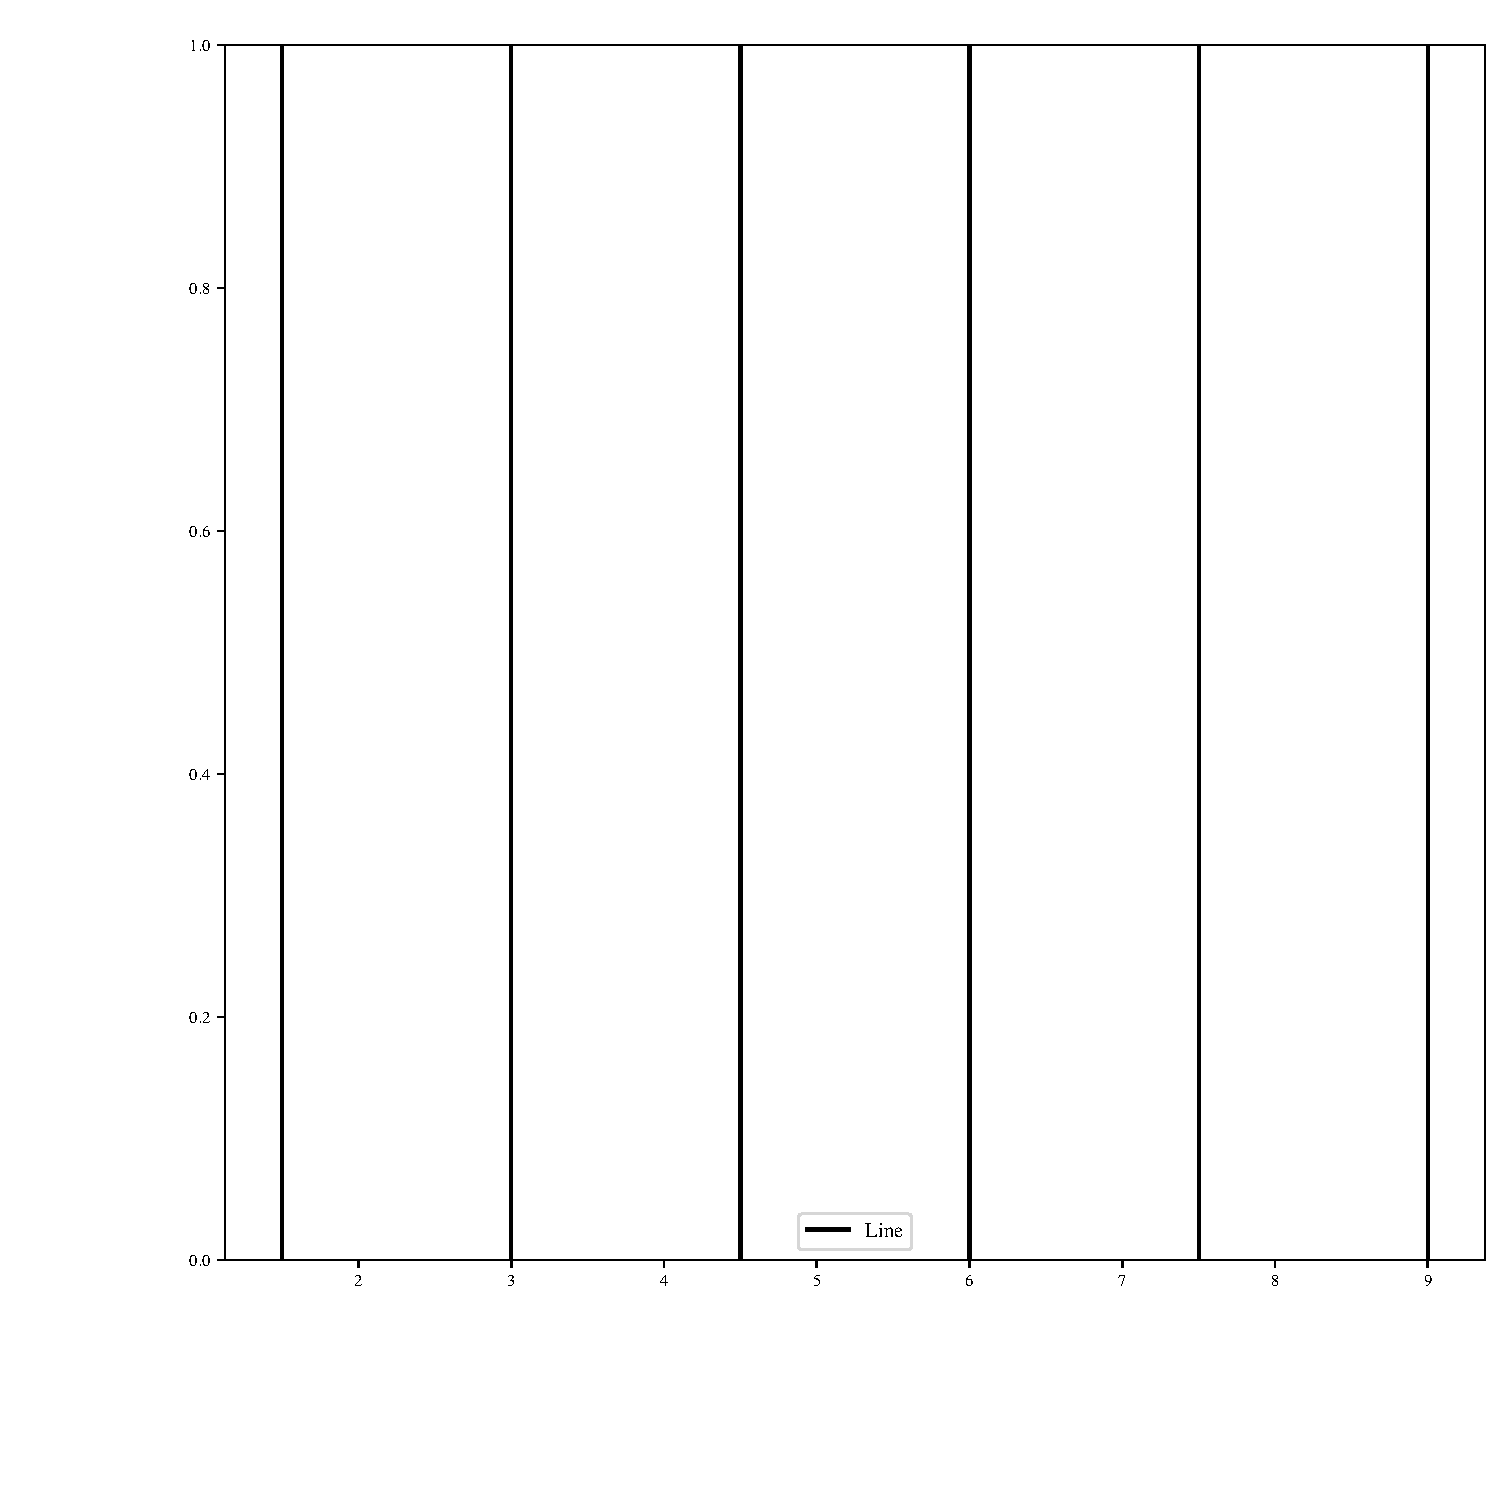
\includegraphics[width=.5\textwidth]{buffon.pdf}
    \caption{Sample Buffon needle experiment. 100 needles are dropped on a 10 $\times$ 10 cm area with lines spaced 1.5~cm apart. If a needle lands on a line it is recorded and coloured blue, if it does not land on a line it is coloured red. This simulation gave a value of $\pi$ $\approx$ 3.10.}
    \label{fig:buffon-needle}
    \squeezeup{3.5}
\end{figure}
\FloatBarrier

If a given problem cannot use the inverted sampling method, as it may not be possible to get a PDF or analytically invert the CDF, then the rejection method can be used.
The rejection method is essentially a dart throwing method.
This means that points are randomly chosen and compared to the function.
If the point lies under the function then the point is accepted, if it lies above the function then it is rejected.
For example, if a function, $f(x)$ does not have an analytical PDF, we can use a PDF $p(x)$ such that $f(x) < cp(x)$ where c is a constant.
Therefore, if we sample from $p(x)$ and if the point lies under $f(x)$ then it is accepted, else it is rejected.
~\Cref{fig:picircle} shows an example of this process.
\begin{figure}[!htbp]
    \squeezeup{4}
    \centering
    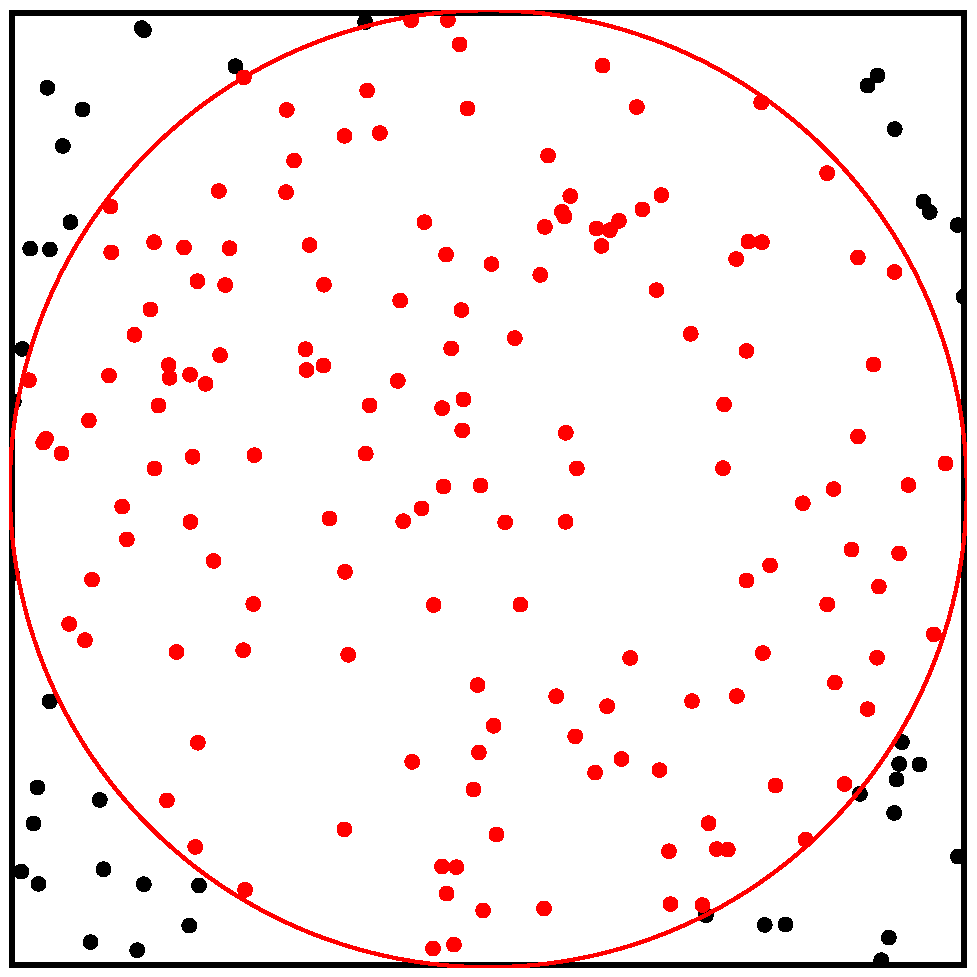
\includegraphics[width=0.3\textwidth]{picirc.pdf}
    \caption{Illustration of the rejection method for determining $\pi$ from the area of a circle inscribed within a square. The ratio of the area of the circle to the square is $\tfrac{\pi}{4}$. Thus, the ratio of darts landing in the circle to those that land outside the circle is $\pi \approx \tfrac{4N_{inner}}{N_{total}}$, where $N_{total}$ is the total number of darts, and $N_{inner}$ is the total number of darts that land in the circle. Using 200 darts gave a value of $\pi \approx 3.12$}
    \label{fig:picircle}
    \squeezeup{7.5}
\end{figure}

\FloatBarrier
One common use of the Monte Carlo method is to randomly sample from a spectrum.
To generate a random sample from a spectrum, first the \gls*{cdf} of the spectrum must be calculated.
This is done by first normalising the \gls*{pdf}, where the \gls*{pdf} in this case is the spectrum itself.
It is normalised such that the sum of the \gls*{pdf} is unity.
The \gls*{cdf} is then just the cumulative sum of the \gls*{pdf}.
Then using the above method as described above, a random number is drawn, $\xi$, and the bracketing values in the \gls*{cdf} are found.
We then interpolate to get the x value corresponding to $\xi$.
\Cref{fig:solar} shows the result of this process for $5\times10^6$ random samples.

\begin{figure}[!htbp]
    \squeezeup{3.5}
    \centering
    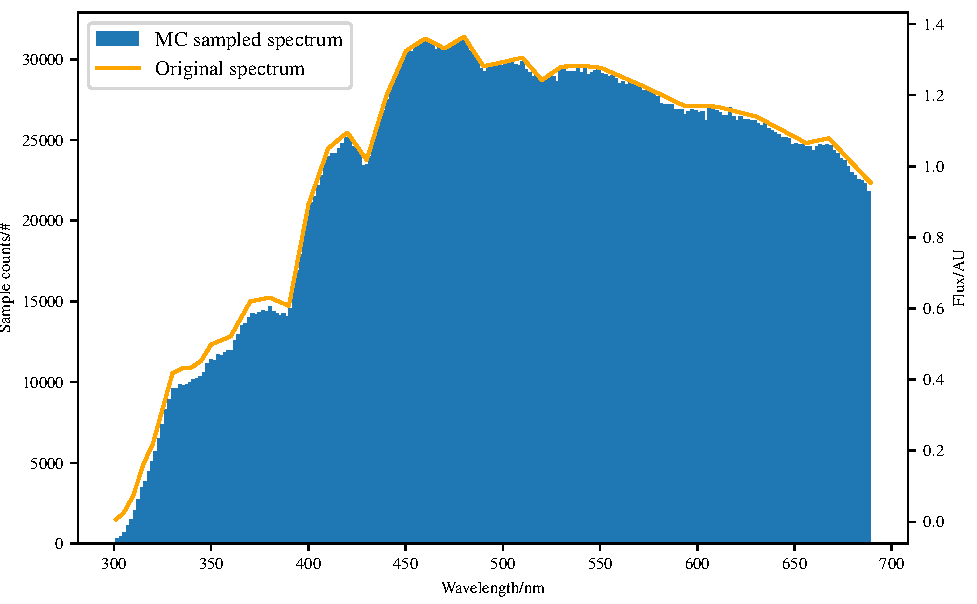
\includegraphics[width=0.75\textwidth]{solar-sample.pdf}
    \caption{Example of randomly sampling from a spectrum. Figure shows 100 random samples drawn to recreate a solar spectrum.}
    \label{fig:solar}
    \squeezeup{3.5}
\end{figure}

The Monte Carlo method is used in various different disciplines. Ranging from use in the financial sector to analyse investments and stocks by simulating the sources of uncertainty which affect their values~\cite{jackel2002monte,finaceprrof}, use in statistical analysis~\cite{wall2012practical}, and in modern computer generated images (see \cref{fig:ray-trace})~\cite{Kajiyarendering,Cookraytracing}. It is also widely used in astronomy~\cite{robitaille2011hyperion,harries2014torus} and medicine~\cite{valentine2011monte,campbell2015monte}, to simulate the propagation of radiation through scattering (turbid) media. This technique, Monte Carlo radiation transfer (MCRT), is what makes up the bulk of this thesis and is described in depth in the following sections.

\begin{figure}[!htbp]
\centering
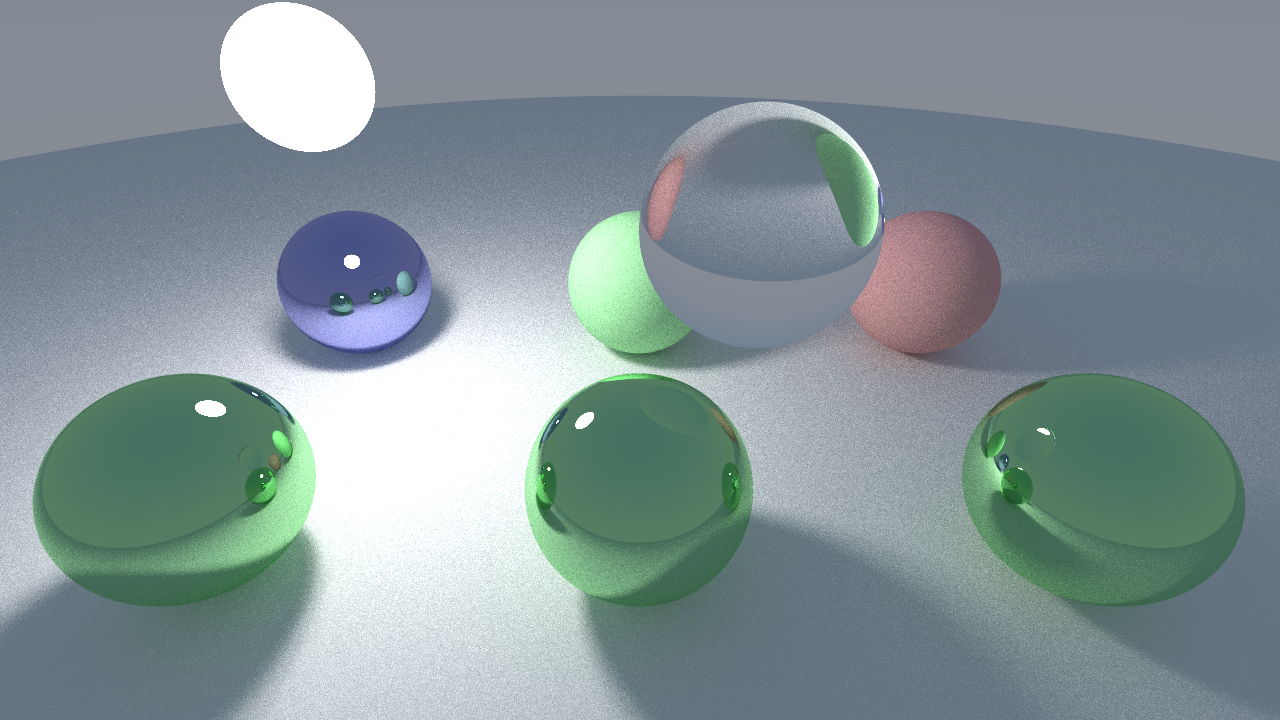
\includegraphics[width=.75\textwidth]{ray-tracing.png}
\caption{Computer generated imagery using ray tracing. The Monte Carlo method is used to ``compute radiance along ray paths between lights and the camera'', to generate CGI images~\cite{pharr2016physically}.}
\label{fig:ray-trace}
\end{figure}


\section{Synopsis and Thesis Objectives}
%sign post chapters

Chapter 2 details the \gls*{mcrt} method which is used for the bulk of this thesis.
Presented in this chapter is the theory behind the MCRT method along with why it is considered the \textit{de-facto} standard in light-tissue interaction modelling.
This chapter also presents a discussion on how the MCRT method is translated into code.
Details of speed up techniques such as parallelisation are also presented.
Finally, to ensure the code is accurate, it is validated against another MCRT code.\\


Chapter 3 details the tissue ablation model developed as part of this thesis.
The tissue ablation model was created to predict the depth of ablation craters in tissue for a given laser power.
The model could also be used to help optimise treatment regimes in cosmetic and medical procedures.
The numerical tissue ablation model consists of 3 numerical methods: MCRT to model the light transport in the tissue, numerical heat model to model the heat diffusion within the tissue, and a numerical tissue damage model to assess the damage to the tissue due to the laser.
The predictive power of the method is demonstrated by the way of optimising spy disposal.
Discussion of the model, alongside validation of the model against theoretical and experimental evidence is presented.\\


Chapter 4 presents an adaptation to the regular Monte Carlo model so it can model wave like properties of photons including diffraction and interference.
The new algorithm is validated against several common experiments that exhibit the wave like behaviour of light, including: diffraction by slits and apertures.
The algorithm is then used to model Bessel beams and shows their ``self-healing'' effect.
Gaussian beams are also modelled using this new algorithm.
The algorithm is also validated against real experimental data, taken by collaborators at the University of Dundee.
Finally the algorithm is used to compare Bessel beams and Gaussian beams in highly turbid media, to determine which beam can image deepest.\\


Chapter 5 details the modelling of a novel biomarker for cardiovascular disease, autofluorescence.
The theoretical groundwork for the biomarker is presented along with discussion of how \gls*{mcrt} can model fluorescence.
Presented alongside this is ameombaMCRT, a Monte Carlo radiation transfer simplex algorithm used to determine concentrations of fluorophores in different layers of tissue for a given spectrum.
Finally, a study of how tissue optics affect the autofluorescent signal is presented. This study investigates the effect of blood, melanin, and skin thickness can have on the autofluorescent signal.


Finally, chapter 6 concludes this thesis and presents possible future avenues of research which could be undertaken.